\documentclass{zc-ust-hw}

\usepackage{lipsum}
\usepackage{circuitikz}
\usepackage{caption} 

\newcommand*{\name}{SalahDin Rezk}
\newcommand*{\id}{202201079}
\newcommand*{\course}{Electric Circuits (ENGR210)}
\newcommand*{\assignment}{Practical Lab 2 Report}

\begin{document}

\maketitle

\begin{enumerate}

  \item
    \begin{figure}[htpb]
      \centering
      \begin{minipage}{0.5\textwidth}
        \centering
        \begin{circuitikz}[american]
          \draw (0,0) to [V, l=128 V] (0,3)
          to [R, l=5 $\Omega$, i=$i_a$] (2,3)
          to [R, l=4 $\Omega$, i=$i_c$] (4,3)
          to [R, l=80 $\Omega$, i=$i_d$] (4,0)
          to [short] (0,0);
          \draw (2,3) to [R, l=60 $\Omega$, i=$i_b$, *-*] (2,0);
        \end{circuitikz}
        \caption{Circuit Diagram}
        \label{fig:circuit-1}
      \end{minipage}%
      \begin{minipage}{0.5\textwidth}
        \centering
        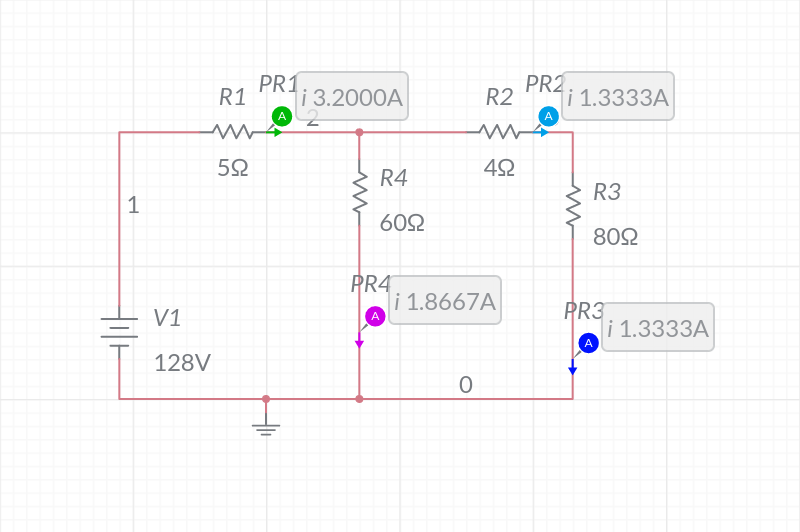
\includegraphics[width=\textwidth]{figures/1699102583.png}
        \caption{Circuit Simulation}
        \label{fig:1}
      \end{minipage}
    \end{figure}

    \begin{align}
      5I_1 + 60(I_1-I_2) &= 128 \\
      60(I_2-I_1) + 4I_2 + 80I_2 &= 0
    .\end{align}
    \begin{align}
      65I_1 - 60I_2 &= 128 \\
      -60I_1 + 144I_2 &= 0
    .\end{align}
    \begin{align}
      I_1 &= 3.20 \\
      I_2 &= 1.33
    .\end{align}
    \begin{align}
      i_a &= I_1 = 3.20 \\
      i_b &= I_1 - I_2 = 1.87 \\
      i_c &= I_2 = 1.33 \\
      i_d &= I_2 = 1.33
    .\end{align}

    \newpage

  \item
    \begin{figure}[htpb]
      \centering
      \begin{minipage}{0.5\textwidth}
        \centering
        \begin{circuitikz}[american]
          \draw (0,0) to [I, l=19 A] (0,3)
          to [short] (2,3)
          to [R, l=5 $\Omega$, i<=$i_a$] (6,3)
          to [controlled current source, l=2$i_b$, invert] (6,0)
          to [short] (0,0);
          \draw (2,3) to [R, l_=40 $\Omega$, i=$i_b$, *-*] (2,0);
        \end{circuitikz}
        \caption{Circuit Diagram}
        \label{fig:circuit-2}
      \end{minipage}%
      \begin{minipage}{0.5\textwidth}
        \centering
        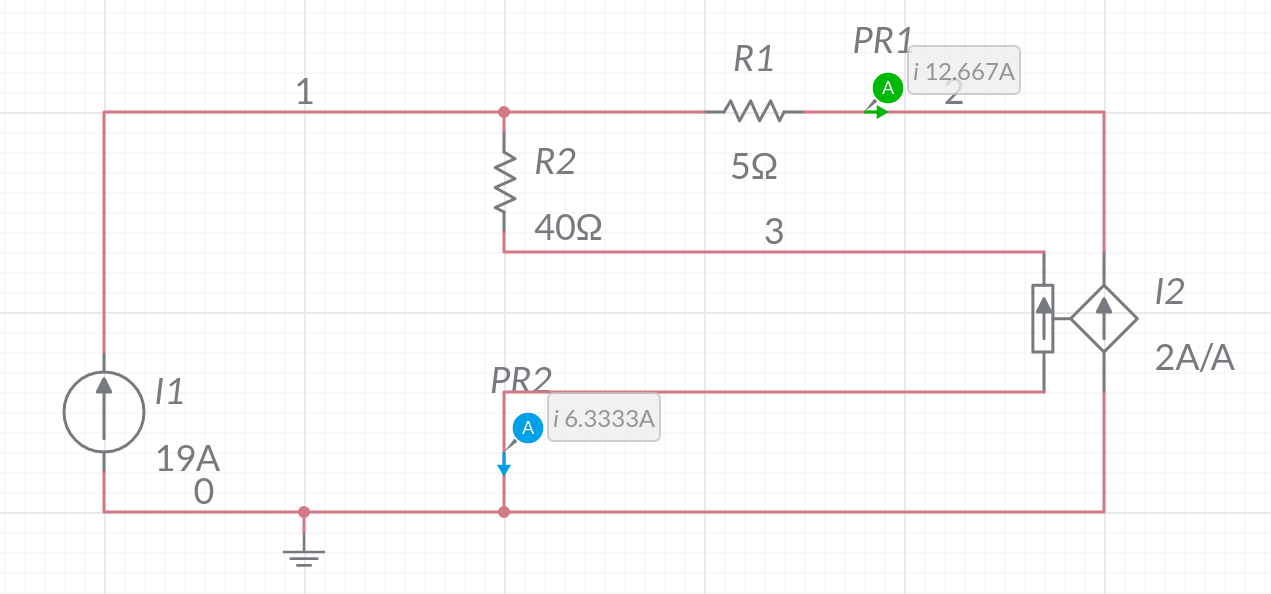
\includegraphics[width=\textwidth]{figures/1699643291.png}
        \caption{Circuit Simulation}
        \label{fig:2}
      \end{minipage}
    \end{figure}

    \begin{align}
      19+i_a&+i_b = 0 \\
      i_a &= 2i_b
    .\end{align}
    \begin{align}
      i_b &= \frac{19}{3} \\
          &\approx 6.33 \\
      i_a &= 2i_b \\
          &\approx 12.67
    .\end{align}

\end{enumerate}

\end{document}
